\documentclass[UTF8]{ctexart}
\usepackage{}
\usepackage{amssymb}
\usepackage{amsmath}
\usepackage{lmodern}

\makeatletter %使\section中的内容左对齐
\renewcommand{\section}{\@startsection{section}{1}{0mm}
  {-\baselineskip}{0.5\baselineskip}{\bf\leftline}}
\makeatother

\title{开发笔记}
\author{Ivan Lin}
\date{\today}
\begin{document}
\maketitle

\section*{Visual Studio}
\noindent Resharper插件\\
alt + o: .h和.cpp文件切换\\
alt + 鼠标: 框选模式\\
ctrl+k + ctrl+c: 注释代码\\
shift+alt+up/down: 框选模式上下\\
ctrl+alt+a: open Command Window\\
ReSharper\_Suspend/ReSharper\_Resume in Command Window: close/open ReSharper\\
lib:静态库,在编译时将库代码加入程序中;dll:动态库,编译时生成一个lib和一个dll,lib用于存放dll中相应接口的索引\\
\section*{计算机图形学}
\noindent 坐标系模拟:拇指x,食指y,中指z。左手系和右手系\\
标准化向量 = 单位向量 = 法线,$\textbf{v}_{norm} = \frac{\textbf{v}}{\textbf{\textbar v\textbar }}$\\
\textbf{a} + \textbf{b} 几何解释:\textbf{a}的头连接\textbf{b}的尾,然后从\textbf{a}的尾向\textbf{b} 的头画一个向量\\
\textbf{a} - \textbf{b} 几何解释:\textbf{a}的尾连接\textbf{b}的尾,然后从\textbf{b}的头向\textbf{a} 的头画一个向量\\
向量点乘:\textbf{a $\cdot$ b}(\textbf{ab}) = \textbf{$a_1b_1+...+a_nb_n$}, 几何解释:\textbf{a $\cdot$ b} = \textbf{\textbar a\textbar \textbar b\textbar }cos$\theta$(两向量夹角)\\
向量投影:\textbf{v}分解为平行和垂直于\textbf{n}的两个分量。\\
\[ \textbf{v}_{||} = \textbf{n}\frac{\textbf{v $\cdot$ n}}{\textbf{\textbar n\textbar }^2} \qquad \textbf{v}_{\bot} = \textbf{\textbar v\textbar } - \textbf{v}_{||}\]
向量叉乘:仅可用于3D向量,$\textbf{a}\times\textbf{b} = \begin{bmatrix} \textbf{a}_y\textbf{b}_z - \textbf{a}_z\textbf{b}_y \\ \textbf{a}_z\textbf{b}_x - \textbf{a}_x\textbf{b}_z \\ \textbf{a}_x\textbf{b}_y - \textbf{a}_y\textbf{b}_x \end{bmatrix}$,几何解释:结果向量垂直于原来两个向量,$|\textbf{a}\times\textbf{b}| = |\textbf{a}||\textbf{b}|sin\theta$\\, $|\textbf{a}\times\textbf{b}| = 0$ 表示\textbf{a}与\textbf{b}平行或有一个为\textbf{0}\\
矩阵转置: \textbf{$M^T$}, 其列由\textbf{M}的行组成,\textbf{${M^T}_{ji}$} = \textbf{$M_{ij}$}\\
\textbf{${(AB)}^T = {B^T}{A^T}$}, 可推广到字符串翻转\\
$P_{camera} = P_{object}M_{object\to world}M_{world\to camera}$\\
线性变换: F(a+b) = F(a)+F(b), F(ka) = kF(a), 则称映射F是线性的(\textbf{aM}满足此条件)\\
仿射变换: 线性变换后接平移, $v^{'} = v\textbf{M} + \textbf{b}$\\
对\textbf{aM}, 求逆变换等价于求矩阵的逆\\
矩阵行列式: $|\textbf{M}|  = \sum_{j=1}^{n}m_{ij}c_{ij} = \sum_{j=1}^{n}m_{ij}(-1)^{i+j}| \textbf{M}^{\{ij\}}|$\\
矩阵的逆: $M(M^{-1}) = M^-1M = I$, 不可逆矩阵又称奇异矩阵,奇异矩阵行列式为0\\
标准伴随矩阵:adj\textbf{M}, M的代数余子式矩阵的转置矩阵。$M^{-1} = \frac{adj\textbf{M}}{|\textbf{M}|}$\\
正交矩阵:\textbf{$MM^{T} = I$}, 旋转和镜像矩阵是正交矩阵。正交矩阵满足:矩阵的每一行都是单位向量,矩阵的所有行相互垂直。\\
Vector4, 齐次坐标。(x, y, z, w)实际代表3D中的(x/w, y/w, z/w)\\
旋转矩阵:描述一个坐标中基向量到另一个坐标基向量的转换。\\
矩阵蠕变:由于浮点数精度有限导致误差积累。\\
欧拉角:heading-pitch-bank约定。\\
万向锁:三个角度不互相独立,一旦选择正负90度为pitch角,就被限制在只能绕竖直轴旋转,失去了一个维度。\\
四元数:\\
几何图元自由度:是无歧义的描述该实体所需信息量的最小数目。\\
射线:是一个有向线段,参数形式:$x(t)=x_0+t\triangle x \quad y(t)=y_0+t\triangle y$,向量记法:$p(t)=p_0 + td$,增量向量d指定了它的长度和方向, 斜截式:$y=mx+b$\\
球和圆:球表面积$S=4\pi r^2$, 球体积$V=\frac{4}{3}\pi r^3$\\
AABB: axially aligned bounding box, 轴对齐矩形边界框, 边垂直于坐标系.使用两个坐标$P_{min}$和$P_{max}$即可表示一个AABB. 变换AABB的方法,一种是重新计算变换物体的AABB, 另一种是变换AABB的八个顶点,然后根据这几个顶点计算新的AABB.\\
OBB: oriented bounding box, 方向矩形边界框。\\
平面: 隐式定义: $\textbf{p}\cdot \textbf{n}=d$, \textbf{n}为平面法向量,垂直于平面,指向方向为平面的正方向; 三个点定义: \textbf{n}通过两个点叉乘并标准化得到,d通过\textbf{n}与其中一个点点乘得到。\\
点集的最佳平面:$\textbf{n}_x=\sum_{i=1}^{n}(z_{i}+z_{i+1})(y_{i}-y_{i+1})\qquad \textbf{n}_y=\sum_{i=1}^{n}(x_{i}+x_{i+1})(z_{i}-z_{i+1})\qquad \textbf{n}_z=\sum_{i=1}^{n}(y_{i}+y_{i+1})(x_{i}-x_{i+1})$, $d=\frac{1}{n}(\sum_{i=1}^{n}p_{i})\cdot \textbf{n}$\\
点到平面的距离: $a=\textbf{q}\cdot \textbf{n}-d$\\
三角形面积: 海伦公式: $A=\sqrt{s(s-l_1)(s-l_2)(s-l_3))}$(s为周长的一半,l为三边长); $A=\frac{||e_1\times e_2||}{2}$(e为三角形的两个边向量)。\\
凸多边形: 对于一个凸多边形,其内角和为$(n-2)180^{\circ}$,判断一个点是否在多边形内,该点与所有顶点的连线组成的角度和为$360^{\circ}$。\\
点\textbf{q}在2D隐式直线上的投影点$\textbf{q'}=\textbf{q}+(d-\textbf{q}\cdot\textbf{n})\textbf{n}$\\
索引三角网格:维护两个列表:顶点表和三角形表;每个顶点包含3D位置,以及纹理映射坐标、表面法向量、光照值等数据;每个三角形由顶点列表的三个索引组成,以及表面法向量、材质等。\\
三种提交方法:顶点缓存:将最近使用的顶点缓存,提交前查询,有则直接使用;三角带:顶点按顺序排布,经常使用退化三角形连接多个三角带;三角扇:与三角带类似,但较不灵活。\\
纹理映射坐标:将位图贴到多边形表面的过程,通常在顶点保存纹理映射坐标,三角形面中其余各点的坐标通过插值计算。\\
表面法向量存储于三角形或顶点中,用于计算光照、进行背面剔除,模拟粒子弹跳等,顶点法向量一般通过平均顶点法向量方法求得。\\
光照值:由顶点维护,用于沿表面的插值,如Gouraud着色。有时候顶点仅保存法向量,渲染时实时计算光照值。\\
三角网格的拓扑是指当在三角网格中不考虑顶点位置与其他几何性质的逻辑连通性时,两个顶点数相同且三角形互联方式一致的三角网格为同拓扑。\\
封闭网格又称流形,其完美覆盖物体表面,网格没有间隙,无法看到三角形背面。\\
拓扑异常会导致网格不封闭,包括:孤立顶点,重复顶点,退化三角形,开放边,超过两个三角形共享的边,重复面。\\
对三角网格的操作都是逐片或者逐顶点的。\\
焊接顶点:将相似的点合为一个,可大量节省内存。\\
面拆分即复制顶点,使边不再被共用。会导致拓扑间断,常用于角和边等几何间断的地方。只拆分,不移动,新的顶点和边是重合的。\\
边缩坍:将边缩减为顶点的方法,常用于网格消减。\\
图形管道数据流概述:建立场景---检测可见性---设置物体级的渲染状态---生成几何体并提交---变换与光照---背面剔除与裁剪---投影到屏幕空间---光栅化---像素着色\\
帧缓存(frame buffer?)一般指用来保存我们正渲染图像的那块内存。\\
坐标空间在渲染管道中的顺序:物体空间,存储顶点位置和表面法向量---世界空间,存储光照值---摄像机空间---裁剪空间(标准视体空间),其对应的矩阵称裁剪矩阵,裁剪矩阵将坐标值除以w,为透视投影做准备---屏幕空间,计算得到x和y,z用于透视校正。\\
光照的类型:点光源(灯泡火把),平行光(太阳光),聚光灯(放映机、车头灯),环境光(阳光漫反射)。\\
标准光照方程:$C_{lit}=C_{spec}+C_{diff}+C_{amb}$,$C_{spec}$是镜面反射分量,$C_{diff}$是散射分量,$C_{amb}$ 是环境分量。物体外观主要取决于:物体表面的性质,即材质属性;表面的方向和朝向(单位法向量);各光源属性;观察者位置。\\
镜面反射分量:由光源直接经物体表面反射入眼睛的光线。\\
Phong模型:$c_{spec}=(cos\theta )^{m_{gls}}s_{spec}\otimes m_{spec}=(v\cdot r)^{m_{gls}}s_{spec}\otimes m_{spec}$。$m_{gls}$为材料光泽度,也称Phong指数,控制光斑的范围,小的值带来大而平滑的光斑,大的值带来小而亮的光斑;$m_{spec}$为材料的反射颜色,控制光斑的强度;$s_{spec}$是光源的镜面反射颜色,控制光本身的色彩与强度。\\
Blinn模型:$c_{spec}=(n\cdot h)^{m_{gls}s_{spec}\otimes m_{spec}}$\\
漫反射服从Lambert法则:反射光强正比于法向量与光线夹角的余弦,$c_{diff}=(n\cdot l)s_{diff}\otimes m_{diff}$,n 为法向量,l为指向光源的单位向量,$m_{diff}$为材料的散射色,$s_{diff}$为光源散射色,一般与光源镜面色$s_{spec}$ 相同。\\
环境光:$c_{amb}=g_{amb}\otimes m_{amb}$,$m_{amb}$为材质的环境光分量,等于漫反射分量,$g_{amb}$为场景的环境光值。\\
光的衰减:$i(d)=1, d\leq d_{min}; i(d)=\frac{d_{max}-d}{d_{max}-d_{min}}, d_{min}<d<d_{max}; i(d)=0, d\geq d_{max}$\\
合成光照方程:$c_{lit}=\sum_{j=1}^{n}i_j(max(n\cdot h_j,0)^{m_{gls}}s_{j_{spec}}\otimes m_{spec}+max(n\cdot l_j,0)s_{j_{diff}}\otimes m_{diff})+g_{amb}\otimes m_{amb}$,因为有多个光源,所以要对每个光源的镜面反射和漫反射进行相加,环境光则不用。\\
雾化:0-1的雾浓度,$c_{fogged}=c_{lit}+f(g_{fog}-c_{lit})$,其中$c_{lit}$为计算光照后的物体表面颜色,f为雾浓度,$g_{fog}$为全局雾颜色,$c_{fogged}$为最终结果。\\
flat着色(逐多边形)和Gourand着色(逐顶点):flat着色效果不佳,暴露出模型的多边形本质。Gourand着色效果较好,是常用的着色手段。\\
缓存:帧缓存存储每个像素的色彩;z-buffer存储像素的深度信息。\\
纹理图是铺在物体表面上的位图,使用纹理映射可在texel(纹理图中的一个像素)级别控制颜色,优于顶点或三角形级别控制。uv坐标。\\
生成与提交几何体:LOD(细节层次)选择:渐进式网格生成,使用网格消减技术;向API投送几何体:API不需要超过三角形级别的数据。\\
变换与光照:物体空间顶点位置变换到裁剪空间,计算光照,计算顶点雾浓度,产生纹理映射坐标,计算骨骼动画顶点值。\\
背面剔除与裁剪:剔除背向摄像机的三角形,一般根据顶点顺序判断。\\
光栅化:着色,测试,写入。\\
可见面检测VSD:找出最终渲染画面中应绘制的三角形。使用视锥探测包围盒。\\
四叉树:用于2D中的自适应空间分层(将平面分成四个象限,每个象限又可以细分,直到某个节点完全处于某个象限中),八叉树是四叉树的3D延伸。\\
\section*{OpenGL}
\noindent OpenGL是Khronos组织制定并维护的规范,但是实现由开发者自己实现(显卡生产商)。\\
OpenGL 3.2以前使用的是立即渲染模式,之后使用的是核心模式(更复杂但更灵活高效)。\\
OpenGL是状态机:由一系列变量描述OpenGL此刻该如何运行,OpenGL状态常称为上下文(Context),我们使用设置选项和操作缓冲来控制上下文进行渲染。\\
为了解决闪屏的问题,OpenGL引入双缓冲机制,前缓冲显示在屏幕上,下一帧渲染在后缓冲上执行,然后交换前后缓冲。\\
Shader是运行在GPU上的小程序。in和out关键字定义顶点属性(Vertex Attribute),前一个Shader的out属性可以在下一个Shader中通过in属性获得, uniform定义全局属性,在任何Shader上都可以访问。其运行流程如下图:\\
\begin{center}
  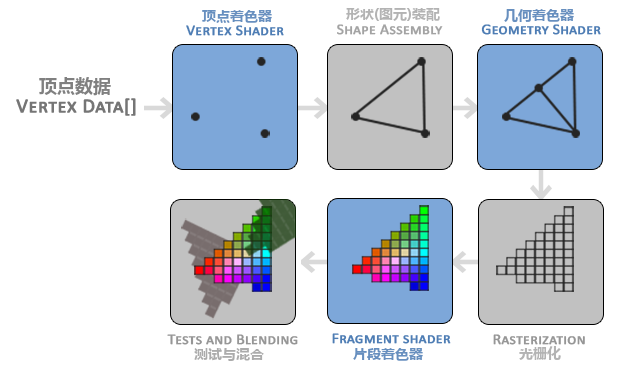
\includegraphics[width=0.8\textwidth]{images/pipeline.png}
\end{center}
\\ 使用纹理坐标获取纹理颜色叫做采样(Sampling),纹理坐标的(0,0)在左下角,(1,1)在右上角。\\
邻近过滤(Nearest): 选取中心点最接近纹理坐标的那个像素;线性过滤(Linear): 基于纹理坐标附件的纹理像素计算出一个插值,近似出这些纹理像素之间的颜色。\\
\section*{Sublime Text 2}
\noindent ctrl+shift+up/down: move line up/down\\
ctrl+alt+up/down: block edit up/down\\
alt+shift+1/2/3/4: change layout\\
ctrl+shift+f: find in files\\
\section*{Swift}
\noindent \textbf{http://blackblake.synology.me/wordpress/?p=29}: Swift里的Optional和Unwrapping\\
\section*{PhotoShop}
\noindent alt+ctrl+c: Resize Canvas\\
alt+ctrl+shift+s: Save for web\\
ctrl+h: show canvas guides; ctrl+mouse drag ruler: add canvas guide\\
\section*{LaTeX}
\noindent \%!Mode:: "TeX:UTF-8": make WinEdt show Chinese\\
\section*{Git}
\noindent gitk file/folder: show commit with file\\
\section*{Windows}
\noindent 放大镜: ctrl+alt+d: 停靠模式; ctrl+alt+l: 窗口模式; win++: 放大; win+esc: 退出放大镜\\
alt+tab, win+tab: 切换窗口\\
win+$\uparrow \downarrow \leftarrow \rightarrow$ : 放大/还原/左置/右置窗口。\\
win+space/d: 透明化/最小化所有窗口。\\
\section*{JavaScript}
\noindent JavaScript组成: ECMAScript, DOM:针对XML文件的操作接口, BOM:浏览器对象模型,HTML5标准化\\
浮点数误差:0.1 + 0.2 = 0.300000000004,通过x10法解决\\
JS没有函数签名,所以不能重载,可通过判断输入参数(arguments, callee, caller)的个数模仿重载, 而且也没有接口继承. P.S.函数签名: 包含函数名、参数类型、类名以及空间名等\\
JS对象类型:基本类型和引用类型,不可以直接操作内存空间,操作的是对象的引用。\\
JS函数参数是值传递。\\
JS没有块级作用域,即if/for循环中的变量不会在循环结束后销毁。局部环境:function, 全局环境\\
垃圾回收机制:1. 标记清除;2. 引用计数(会有循环引用的问题)\\
引用类型不是类,类是定义同一类所有对象的变量和方法的蓝图或原型,有接口和结构。\\
推荐使用对象字面量语法定义对象,因为更有封装概念,并且可以“重载”构造函数。\\
JS的数组可以同时储存任何类型的数据,且长度动态增长。var colors = new Array(); || var colors = ["red", "green", "blue"];\\
JS的数组length是非只读的,修改该值会删除相应的元素。\\
splice函数: splice(0, 2): 删除数组中的前两项; splice(2, 0, "red", "green"): 从位置2插入"red"和"green"; splice(2, 1, "red"): 删除位置2的元素,并插入"red"\\
JS的函数实际上是Function类型的实例。\\
解释器会先读取函数声明(function sum(){};)(函数声明提升),但函数表达式(var sum = function(){};)(又称匿名函数(Lambda))需要到相应的行才会执行。\\
this引用的是函数据以执行的环境对象。\\
不属于其他任何对象的属性和方法都属于Global对象的属性和方法,如isNaN().\\
eval()函数传入完整的JS代码。\\
代码注入:\\
对象中数据属性的四个特性:[[Configurable]] [[Enumerable]] [[Writable]] [[Value]], 使用defineProperty(obj, "propertyName")函数修改。\\
\_year表示只能通过对象方法访问的属性,需要在defineProperty(obj, "year")中定义getter和setter函数。\\
hasOwnProperty(name)只在有实例属性的时候返回true(对应的是hasPrototypeProperty(name)), "name" in obj在原型属性和实例属性都返回true。\\
JS通过原型链实现继承, 具体实现为借用构造函数+原型链的寄生组合继承。\\
闭包是指有权访问另一个函数作用域中的变量的函数。创建闭包的常用方式就是在函数内部创建另一个函数。闭包通过作用域链继续retain外部函数的实例,直到闭包函数结束调用或解除引用才会释放外部函数的实例。\\
JS通过闭包模仿块级作用域和私有变量。\\
BOM的核心是window对象,代表Global对象。\\
top.frames[0]代表最外层框架,frame中包含window的集合。\\
alter(), confirm(), prompt()用于弹出对话框。\\
\section*{编译原理}
\noindent 有限自动机$\rightarrow$词法分析,上下文无关文法$\rightarrow$语法分析\\
左值: 一个名字所代表的单元地址;右值: 一个名字的值,变量既持有左值也持有右值,常数和带算符的表达式只有右值;=左边的名字必须持有左值,右边的名字只需持有右值。\\
上下文无关文法:它所定义的语法范畴是完全独立于这种范畴可能出现的环境的。包括四个组成部分:一组终结符号,一组非终结符号,一个开始符号,一组产生式。\\
最左/右推导: 从$\alpha\Rightarrow\beta$的最左非终结符号进行替换,$\Rightarrow$代表一步推导。\\
如果一个文法存在某个句子对应两棵不同的语法树,则称这个文法是二义的。\\
形式语言:0型>1型>2型>3型。0型又称短语文法,图灵机,是递归可枚举的;1型又称上下文有关文法;2型称上下文无关文法;3型称右线性文法或正规文法。\\
词法分析器输入源程序,输出单词符号,常表示成(单词种别,单词符号的属性值)。单词符号一般分为关键字、标识符、常数、运算符、界符。\\
词法分析流程:输入,预处理:将源程序存入缓冲区,去除多余空格、换行、注释等----超前搜索:扫描到能够确定单词类型的字符为止,如, = 等符号----状态转换图表述识别流程。\\
正规式(正则表达式)和正规集。确定有限自动机(DFA)M是一个五元式,$M=(S,\Sigma,\delta,s_0,F)$,其中S是一个有限集,它的每个元素称为状态; $\Sigma$是一个有穷字母表,其每个元素称为一个输入字符; $\delta$是一个从$S\times \Sigma$ 至S的单值部分映射。$\delta(s,a)=s^{'}$意味着,当现行状态为s,输入字符为a时,转换到下一状态$s^{'}$;$s_0\in S$,是唯一的初态;$F\subseteq S$, 是一个终态集(可空)。\\
非确定有限自动机(NFA)。\\
一个描述词法分析器的LEX程序由一组正规式以及与每个正规式相应的一个“动作”组成。\\
语法分析是编译过程的核心,一般使用自上而下分析法或自下而上分析法。从输入符号串到句子的过程。\\
自上而下就是从文法的开始符号出发,向下推导,推出句子,一般使用递归。\\
自上而下文法要消除回溯和左递归,LL(1)文法:第一个L表示从左到右扫描输入串,第二个L表示最左推导,1表示每步只需向前查看一个符号。递归下降分析器。\\
LL(1)文法常用预测分析表实现。
\end{document}
